\subsection{\gls{vi}}
When using topic models and other Bayesian models, it is computationally infeasable to compute the posterior, which means approximation is needed. 
Approaches today use two types of inference algorithms to estimate this; sampling and optimization approaches.

A widely used sampling approach is the MCMC algorithm Gibbs Sampling.
Gibbs sampling approximates the posterior distribution by trying to infer hidden structure by iteratively recalculate the state of each node based on its neighbors or similar nodes in a Bayesian network.

\gls{vi} is used to solve inference with optimization.
In \gls{vi}, we have the initial variational parameters $\nu_{init}$ in which we want approximate the true posterior distribution $p(z|\textbf{x})$ where $z$ is the hidden variables and $x$ is the observations.
We do the approximation by fitting variational parameters $\nu$, to mimize the distance between initial distribution $v$ and $\nu^*$ where $\nu^*$ is the distribution that is closest to $p(z|\textbf{x})$.
In \autoref{fig:vi}, we can see a visualization of this where we want to optimize the variational parameters to minimize the distance be the true posterior distribution.
In \autoref{fig:vi}, $q(z; \nu)$ is a family of variational distributions over the latent variables which is different instances of the hidden variables $z$.
Our goal is to fit the variational paramaters $\nu$ to estimate the hidden variables that are closest to $p(z|\textbf{x})$

\begin{figure}
	\centering
	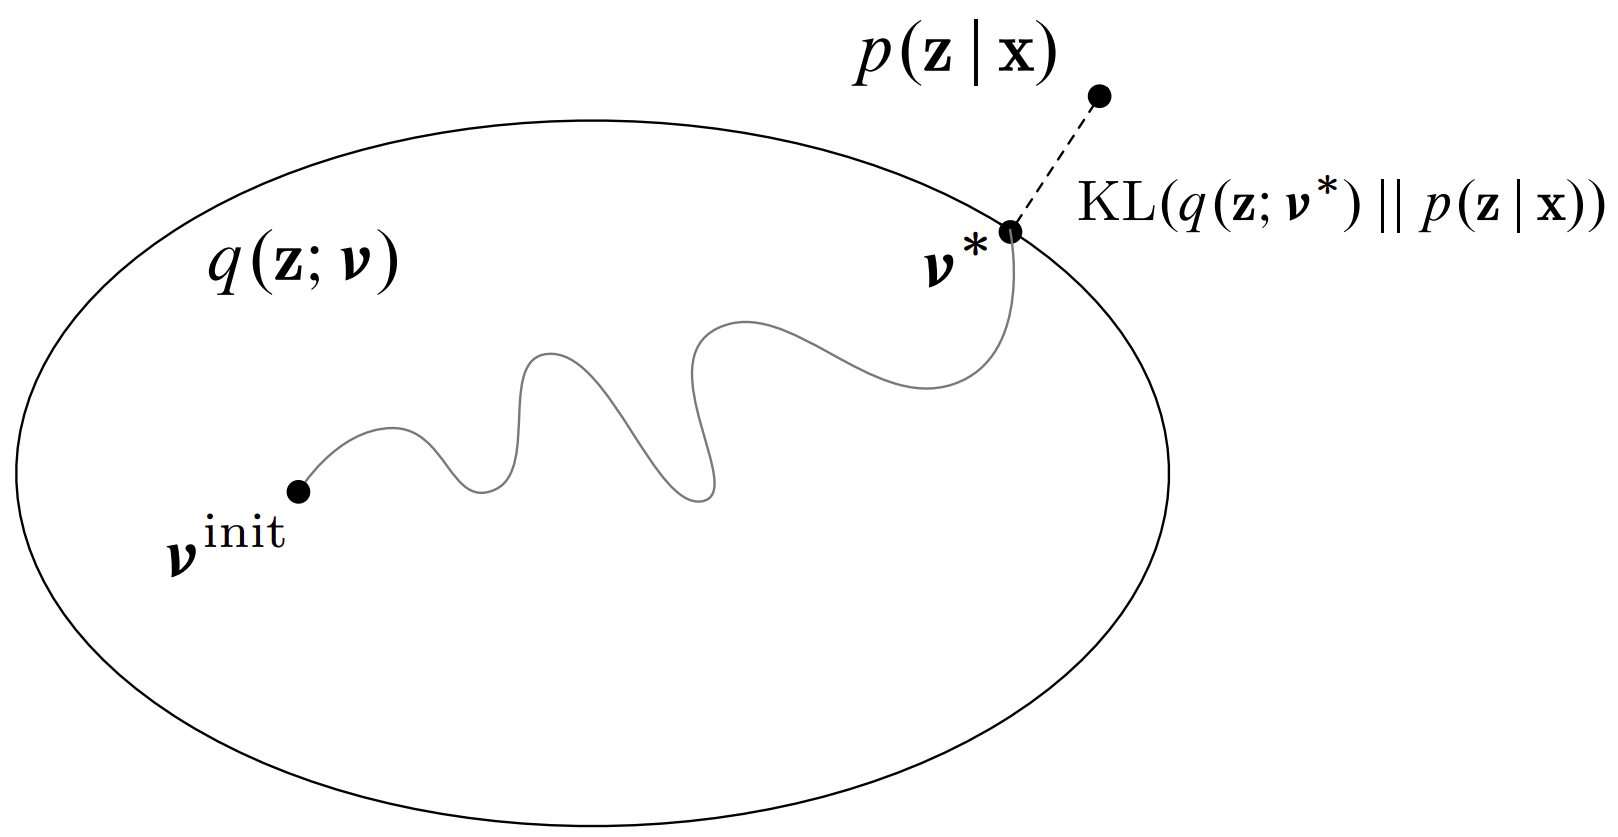
\includegraphics[width=0.5\textwidth]{figures/vi_illustration.png}
	\caption{Illustration of \acrlong{vi}}
	\label{fig:vi}
\end{figure}

\subsubsection{LDA learning}
We use an implementation of the LDA which is based on \cite{blei2010online}, where \citeauthor{blei2010online} present a way of training the LDA using \gls{vi}.
They do this by using Stocastic \gls{vi}, which also outperforms batch learning.
To do  
